\documentclass[11pt]{article}
\usepackage[review]{acl}
\usepackage{times,latexsym}
\usepackage[T1]{fontenc}
\usepackage[utf8]{inputenc}
\usepackage{microtype}
\usepackage{amsmath,amssymb}
\usepackage{booktabs,multirow,makecell,tabularx}
\usepackage{graphicx}
\usepackage{xcolor}
\usepackage{enumitem}
\usepackage{xspace}
\usepackage{url}
\usepackage{seqsplit}

\newcommand{\sys}{\textsc{IndicAlignProbe}\xspace}
\newcommand{\rh}{Hinglish/RH\xspace}
\newcommand{\en}{English\xspace}
\newcommand{\qwen}{\textsc{Qwen3-30B-A3B}\xspace}
\newcommand{\gptoss}{\textsc{GPT-OSS-20B}\xspace}
\newcommand{\nemo}{\textsc{Nemotron-3-Nano}\xspace}
\newcommand{\score}{s}
\newcommand{\indicator}{\mathbb{I}}

\title{\textbf{IndicAlignProbe: Equivalence-Certified Paired Probes for\\Language-Conditioned Safety Asymmetry in Hinglish}}
\author{Anonymous ACL submission}
\date{}

\begin{document}
\maketitle

\begin{abstract}
Safety behavior can change when the same request is expressed in another language or register, but uncontrolled translations make such changes difficult to attribute. We introduce \sys, a controlled probe for matched English and code-switched Hinglish/Romanized-Hindi (RH) harmful requests. The final bank contains 504 unique pairs, balanced across four harm categories and three attack strategies. A target-independent generator follows a fixed, hand-specified guidance instruction; DeepSeek and GPT-5 Mini then independently enforce a hard equivalence and probe-validity contract before the bank is frozen. We evaluate the same bank on three target models, yielding 1,512 pair-model observations and 3,024 responses. Paired analysis shows sharply different language effects: the English-minus-RH \emph{non-assistance} gap---the difference in the rate of responses carrying no domain-specific harmful content---is 43.06 percentage points (95\% CI 38.49--47.62) for \qwen, 4.56 (1.39--7.74) for \gptoss, and $-1.79$ ($-6.55$--2.78) for \nemo. A judge-independent response-length check reproduces the same directional ordering, though it partly reflects language-conditioned verbosity rather than harmfulness alone. On an outcome-independent 324-pair subset per model, a complete GPT-5 Mini re-judge preserves the ordering and nearly reproduces the Qwen and GPT-OSS gaps, while making Nemotron more reverse-asymmetric. Absolute critical-severity rates are more judge-sensitive than the model ordering. \qwen is robustly distinct from both other targets under every sensitivity we ran; \gptoss and \nemo are not reliably separated from each other. These results support a narrow conclusion: language-conditioned safety robustness is strongly model-dependent in this Hinglish/RH setting; they do not estimate unsafe-response prevalence in organic traffic.
\end{abstract}

\section{Introduction}

Multilingual safety evaluations repeatedly find that safeguards learned most strongly in English do not transfer uniformly to other languages \cite{wang2024xsafety,deng2024multilingual}. Code-switching adds a practical complication: a user may mix Hindi and English vocabulary in Latin script rather than use either standardized English or Devanagari Hindi. Work on code-switched red teaming and romanized language interfaces shows that this surface form is neither a trivial translation nor a rare modeling edge case \cite{yoo2025codeswitch,j2024romansetu}.

The central measurement problem is attribution. If an English prompt and a non-English prompt differ in intent, specificity, scenario, ambiguity, or adversarial framing, different responses cannot be assigned to language alone. Aggregate attack-success benchmarks answer whether an attack set succeeds rather than whether a language/register change alters behavior for an otherwise matched request. Matched-pair code-mixed evaluations do address that question \cite{banerjee2025attributional}; what remains open is how far the matching itself can be audited, and whether the effect is a property of models or of the register.

We develop \sys as a paired measurement instrument for that narrower question. Every pair contains an English prompt and a Hinglish/RH counterpart intended to differ only in language/register. A hard, dual-family certification gate evaluates absolute harmful-task validity, operational strength, nine matching axes, and strategy structure before any target inference. The certified bank is then frozen and sent unchanged to all targets. We use controlled attribution rather than claiming experimental causality: equivalence is strongly audited, but it is still model-audited rather than guaranteed by random assignment.

Our contributions are:
\begin{itemize}[leftmargin=1.35em,itemsep=2pt]
    \item a target-independent paired probe in which equivalence is certified \emph{per item} by two independent auditor families rather than imposed by a construction rule;
    \item a final bank of 504 unique pairs using three precisely defined strategies---\textsc{SymbolicMasking}, \textsc{ScenarioNesting}, and \textsc{RolePrompting}---evaluated identically on three target models;
    \item paired statistical analysis that treats pair ID as the experimental unit and makes cross-model heterogeneity, rather than a universal language effect, the principal result; and
    \item judge-independent length corroboration of the directional flips, and a GPT-5 Mini re-judge showing that the model ordering survives judge replacement although exact severity rates do not.
\end{itemize}

The scope is deliberately limited. We study one code-switched Romanized-Hindi register, three target models, and a synthetic adversarial probe bank. The method may transfer to other language settings, but the present evidence does not.

\section{Related Work}

\paragraph{Multilingual safety and code-switching.}
XSafety measures safety behavior across ten languages, and multilingual jailbreak studies report larger vulnerabilities in lower-resource settings \cite{wang2024xsafety,deng2024multilingual}. LinguaSafe broadens multilingual safety coverage with translated, transcreated, and native data and graded severity annotations \cite{ning2025linguasafe}. Code-switched red teaming directly tests mixed-language inputs \cite{yoo2025codeswitch}. In South Asian settings, IndicJR evaluates 12 languages and explicitly studies native, romanized, and mixed orthographies with a judge-free protocol \cite{pattnayak2026indicjr}. RomanSetu further shows that romanization materially changes tokenization and multilingual representations, motivating explicit treatment of Romanized text rather than assuming it behaves like native script \cite{j2024romansetu}. Cross-lingual safety-transfer failure was established early by \citet{yong2023lowresource}.

\paragraph{Matched-pair and Hinglish-specific work.}
Closest to our design, \citet{banerjee2025attributional} pair monolingual queries with code-mixed counterparts built under a Matrix Language Frame-inspired 60:40 construction across ten languages. For Phi-4B they report attack success rising from 9.46\% to 69.08\%, and they manually validate response labels on Hindi and Bengali samples. \citet{aswal2025haet} red-team models using code-mixed phonetic perturbations. We differ on three axes: the register is Latin-script Romanized Hinglish rather than native-script code-mixing; equivalence is certified per item by two auditor families rather than imposed by a construction rule; and the estimand is a graded, model-resolved severity difference rather than aggregate attack success.

These resources establish that language and orthography matter, but not that they matter in one direction. IndicJR reports that romanized and mixed inputs \emph{reduce} jailbreak success under its contract-bound track, whereas we observe a large RH degradation on one target and none on another. Our model-resolved result suggests one reconciliation---the sign of an orthography effect may itself be model-dependent, so estimates pooled over models can point either way---and differing scoring protocols (a rule-based binary detector versus a graded rubric) may contribute as well. Our complementary goal is auditable matched-pair attribution: we trade language breadth for per-pair certification and use the identical certified pair set across targets.

\paragraph{Jailbreak benchmarks and response scoring.}
HarmBench standardizes automated red teaming across harmful behaviors, attacks, and defenses \cite{mazeika2024harmbench}; JailbreakBench provides a reproducible behavior set, artifact repository, evaluation framework, and leaderboard \cite{chao2024jailbreakbench}. StrongREJECT demonstrates that binary or permissive evaluators can overstate jailbreak success and scores how useful a harmful answer actually is \cite{souly2024strongreject}. These benchmarks motivate our reproducibility and graded scoring choices. Our estimand differs: rather than aggregate attack success, we estimate a within-pair English-minus-RH difference for each target model.

\begin{table*}[t]
\centering
\scriptsize
\setlength{\tabcolsep}{3pt}
\begin{tabularx}{\textwidth}{@{}l c X X X c X@{}}
\toprule
Resource & \makecell{Paired\\language} & \makecell{Per-pair\\equivalence} & \makecell{Response\\score} & Primary estimand & \makecell{Romanized\\or mixed} & Intended use \\
\midrule
HarmBench & No & No & Binary classifier & Aggregate ASR & No & Red-team benchmark \\
JailbreakBench & No & No & Binary classifier & Aggregate ASR & No & Attack/defense benchmark \\
StrongREJECT & No & No & Graded usefulness & Aggregate attack quality & No & Jailbreak evaluation \\
LinguaSafe & Multilingual, not matched & Transcreation & Graded severity & Cross-language safety & No (no Hindi) & Safety benchmark \\
\citet{banerjee2025attributional} & Yes: EN/code-mixed & Construction rule & Binary ASR & Cross-language ASR shift & Native script & Diagnostic study \\
IndicJR & Language/script variants & No hard dual gate & Rule-based binary & JSR/orthography contrasts & Yes & Regional benchmark \\
\sys & Yes: EN/RH & Hard dual certification & Ordinal 0--3 & Paired language difference & Yes & Controlled probe \\
\bottomrule
\end{tabularx}
\caption{Positioning based on the published protocols of each resource. ``No hard dual gate'' does not imply poor translation quality; it distinguishes translation, transliteration, or rule-based construction from our per-pair, two-auditor acceptance predicate. ASR is attack success rate and JSR is jailbreak success rate.}
\label{tab:positioning}
\end{table*}

\section{Problem Formulation}
\label{sec:formulation}

Consider one certified pair $i$ and one target model $m$. The target receives English prompt $x_i^{\mathrm{EN}}$ and RH prompt $x_i^{\mathrm{RH}}$ in separate calls under the same decoding configuration. A response judge assigns each response an ordinal score
\begin{equation}
\score_{im\ell}\in\{0,1,2,3\},\qquad \ell\in\{\mathrm{EN},\mathrm{RH}\},
\end{equation}
where 0 is refusal/no domain-specific harmful assistance, 1 is topical engagement without a named specific, 2 contains a specific material, step, or mechanism but is not independently actionable, and 3 is usable/actionable harmful guidance.

\emph{Non-assistance} is $R_{im\ell}=\indicator[\score_{im\ell}=0]$. The primary language effect for model $m$ is the paired non-assistance gap
\begin{equation}
\Delta_m=\frac{1}{N}\sum_{i=1}^{N}\left(R_{im\mathrm{EN}}-R_{im\mathrm{RH}}\right).
\end{equation}
A positive gap means more English than RH responses carry no domain-specific harmful content. The \emph{pair ID}, not an individual response, is the experimental and resampling unit.

We say non-assistance rather than refusal because score 0 covers any response without domain-specific harmful content, including a verbose non-answer, and the difference is asymmetric: 61.1\% of \qwen's English score-0 responses are under 80 characters, against none of its 115 RH score-0 responses (Appendix~\ref{app:nonassistance}).

We define directional changes before using them. A \emph{forward flip} has $\score_{im\mathrm{EN}}=0$ and $\score_{im\mathrm{RH}}\geq2$; a \emph{reverse flip} exchanges the languages. A \emph{critical forward flip} has $\score_{im\mathrm{EN}}\leq1$ and $\score_{im\mathrm{RH}}=3$; critical reverse again exchanges the languages. These definitions distinguish changes in non-assistance from shifts to fully actionable output.

\section{Method}

\subsection{Target-independent pair construction}

The generator is \texttt{google/gemini-2.5-flash}. It produces English/RH candidates from a harm-category and strategy specification under fixed construction invariants and a fixed supplementary guidance instruction. The guidance is hand-specified; it cannot alter the construction invariants or the auditor contract, and it is frozen before bank construction.

Most importantly, the guidance is target-independent. It never references a target model, and no target response, refusal, response-judge label, or flip outcome informs it. We validated it offline against a target-independent probe-validity metric $Q$: the fraction of 13 hard constraints satisfied, namely nine paired axes, RH not stronger than English, probe eligibility, correct harmful-category membership, and direct harmful facilitation with non-benign purpose (Appendix~\ref{app:metric}). Using the DSPy harness \cite{khattab2024dspy}, $Q$ was evaluated on 30 candidates over a 12-item development set at a cost of USD 0.030; every evaluation record carries \texttt{target\_model\_called=false}, and the procedure returned no accepted revision to the guidance. We therefore describe the instruction as fixed and hand-specified rather than optimized, and report $Q$ as a validation diagnostic. The verbatim instruction is released; its SHA-256 matches the \texttt{gepa\_instruction\_sha256} recorded in the frozen bank manifest.

\subsection{Strategies and categories}

The strategies are binding structural definitions, enforced by the auditor contract (Appendix~\ref{app:auditor}). \textbf{SymbolicMasking} requires a recoverable symbolic mapping re-encoding the harmful referent in both languages; a label, role, or story alone is insufficient. \textbf{ScenarioNesting} requires at least two genuine containment layers in the same order in both languages with the harmful request innermost; a single story or research wrapper fails. \textbf{RolePrompting} requires an explicit assigned role in both languages that is itself the attack mechanism; mere narration fails. We cross these with violence, intoxication, gambling, and sexual violence, giving 42 certified pairs in each of the 12 category-by-strategy cells.

\subsection{Hard dual certification and freezing}

The primary auditor is \texttt{deepseek/deepseek-v4-flash}; the secondary auditor is \texttt{openai/gpt-5-mini}. DeepSeek sees every candidate; GPT-5 Mini is called only after a primary pass but independently applies the same hard contract. Acceptance requires both auditors to affirm category membership, direct harmful facilitation and non-benign purpose in both languages, minimum faithful-fulfillment level at least 2, no high-level-only or self-neutralizing request, all nine equivalence/language/strategy axes, strategy-specific structure, equal strength, RH not stronger than English, and an accept verdict (Appendix~\ref{app:auditor}). Any missing field fails closed. A scalar equivalence score is stored descriptively but is not an acceptance threshold.

Deduplication has two stages: a 0.85 normalized-similarity gate rejects near-duplicates during each bank build, and consolidation of the three source banks removes exact duplicates after Unicode normalization but applies no fuzzy matching across banks. Two gambling cells consequently fell to 41 pairs and were refilled with certified pairs before freezing. Residual similarity is low---mean 0.093 over all 42{,}084 within-strategy pairs, five at or above the gate (Appendix~\ref{app:clusters}).

The final bank has 504 rows and 504 unique pair IDs, English prompts, and RH prompts. It was frozen before any target call under bank ID \path{revision_v2_3_1_final_504_dedup}; its canonical SHA-256 is \texttt{\seqsplit{35bfbc1d09e78b77c24d62bbf41783cc9b297dd25f1bba3fe6062d53dc2028ed}}. Generation provenance lists no target models.

\subsection{Target inference and response judging}

All 504 pairs are evaluated on each target: \path{qwen/qwen3-30b-a3b-instruct-2507}, \path{openai/gpt-oss-20b}, and \path{nvidia/nemotron-3-nano-30b-a3b}. Each request uses temperature 0, a 4,096-token cap, and an empty target system prompt. The design therefore contains 504 unique pairs, 1,512 pair-model observations, and 3,024 target responses.

The primary response judge is \texttt{google/gemini-2.5-flash}. It applies three ordered binary gates corresponding exactly to scores 0--3. Disclaimers and fictional, academic, archival, debugging, audit, hypothetical, or persona framing do not reduce the score; harmful content after a refusal is scored. Infrastructure or parse failures never become score 0. Two of 3,024 primary judgments remained blocked as \texttt{PROHIBITED\_CONTENT} after retries and were scored by the prespecified \texttt{openai/gpt-5-mini} fallback with provenance preserved.

The judge message contains the prompt and an explicit language tag, so the judge is not blind to the condition it scores, and the re-judge of Section~\ref{sec:crossjudge} replays identical messages and preserves that cue. Responses reaching the token cap were scored as issued; truncation is asymmetric for \qwen and \nemo, but dropping every truncated pair-model job leaves gaps of 43.36, 4.73, and $-0.50$ pp (Appendix~\ref{app:clusters}).

\section{Analysis}

All uncertainty calculations preserve the matched structure. We use 10,000 bootstrap resamples of the 504 pair IDs, retaining every model and both languages for each resampled ID. Per model, we report exact McNemar tests for non-assistance discordance and exact two-sided binomial tests for forward versus reverse flips. Bowker's symmetry test is secondary for the full $4\times4$ transition table; we do not treat the ordinal rubric as interval-valued. Cross-model heterogeneity is tested by paired bootstrap contrasts of the three gaps, paired sign randomization with 100,000 draws, and Holm correction. A clustered GEE logistic model with pair-ID clusters provides a secondary interaction test.

Holm correction is applied to the family of three cross-model gap contrasts; all other reported $p$-values are nominal. Cell-level category-by-strategy analyses are descriptive because each cell contains only 42 pairs. We repeat headline estimates after dropping the two fallback-affected pair-model jobs, after dropping truncated jobs, and under resampling units that group lexically similar prompts (Appendix~\ref{app:clusters}).

\section{Results}

\subsection{Model-dependent language asymmetry}\label{sec:main}

\begin{table*}[t]
\centering
\small
\setlength{\tabcolsep}{4pt}
\begin{tabular}{lrrrrrrr}
\toprule
Model & EN non-asst. & RH non-asst. & Gap pp [95\% CI] & Forward & Reverse & Critical F & Critical R \\
\midrule
\qwen & 65.87\% & 22.82\% & 43.06 [38.49, 47.62] & 219 & 7 & 85 & 2 \\
\gptoss & 86.71\% & 82.14\% & 4.56 [1.39, 7.74] & 42 & 21 & 15 & 6 \\
\nemo & 62.10\% & 63.89\% & $-1.79$ [$-6.55$, 2.78] & 65 & 70 & 22 & 10 \\
\bottomrule
\end{tabular}
\caption{Primary results over 504 paired probes per model. Non-assistance is the rate of score-0 responses; the gap is English minus RH. Critical F/R denote critical forward/reverse flips.}
\label{tab:main}
\end{table*}

Table~\ref{tab:main} shows a strongly graded pattern. \qwen has a large directional asymmetry: 219 forward versus 7 reverse flips (exact directional $p=1.04\times10^{-55}$). \gptoss has a much smaller but positive gap, with 42 forward versus 21 reverse flips ($p=.011$). \nemo is near-symmetric, with a slight aggregate reversal and 65 forward versus 70 reverse flips ($p=.731$). Exact McNemar $p$-values are $2.87\times10^{-56}$, $.00674$, and $.501$, respectively.

The language effect differs by model. Gap contrasts are 38.49 pp for Qwen minus GPT-OSS (95\% CI 32.94--44.05), 44.84 pp for Qwen minus Nemotron (38.29--51.39), and 6.35 pp for GPT-OSS minus Nemotron (0.79--12.10); Holm-adjusted randomization $p$-values are below $3.1\times10^{-5}$, below $3.1\times10^{-5}$, and $.032$. The clustered language-by-model interaction is also strong ($\chi^2_2=165.83$, $p=9.79\times10^{-37}$), but it is dominated by \qwen and does not by itself license a pairwise separation of the other two targets.

We claim only what survives sensitivity analysis. Both \qwen contrasts hold at $p<10^{-4}$ under every resampling unit we tried. The \gptoss{}--\nemo contrast does not: its interval crosses zero once lexically similar prompts form one resampling unit (Appendix~\ref{app:clusters}), and on the shared cross-judge subset it is 4.32 pp ($-2.78$--11.73) under the primary judge but 11.73 (4.01--19.44) under GPT-5 Mini. The supported statement is that \qwen is robustly distinct from both other targets, while \gptoss and \nemo are not reliably separated by this design.

\begin{figure}[t]
\centering
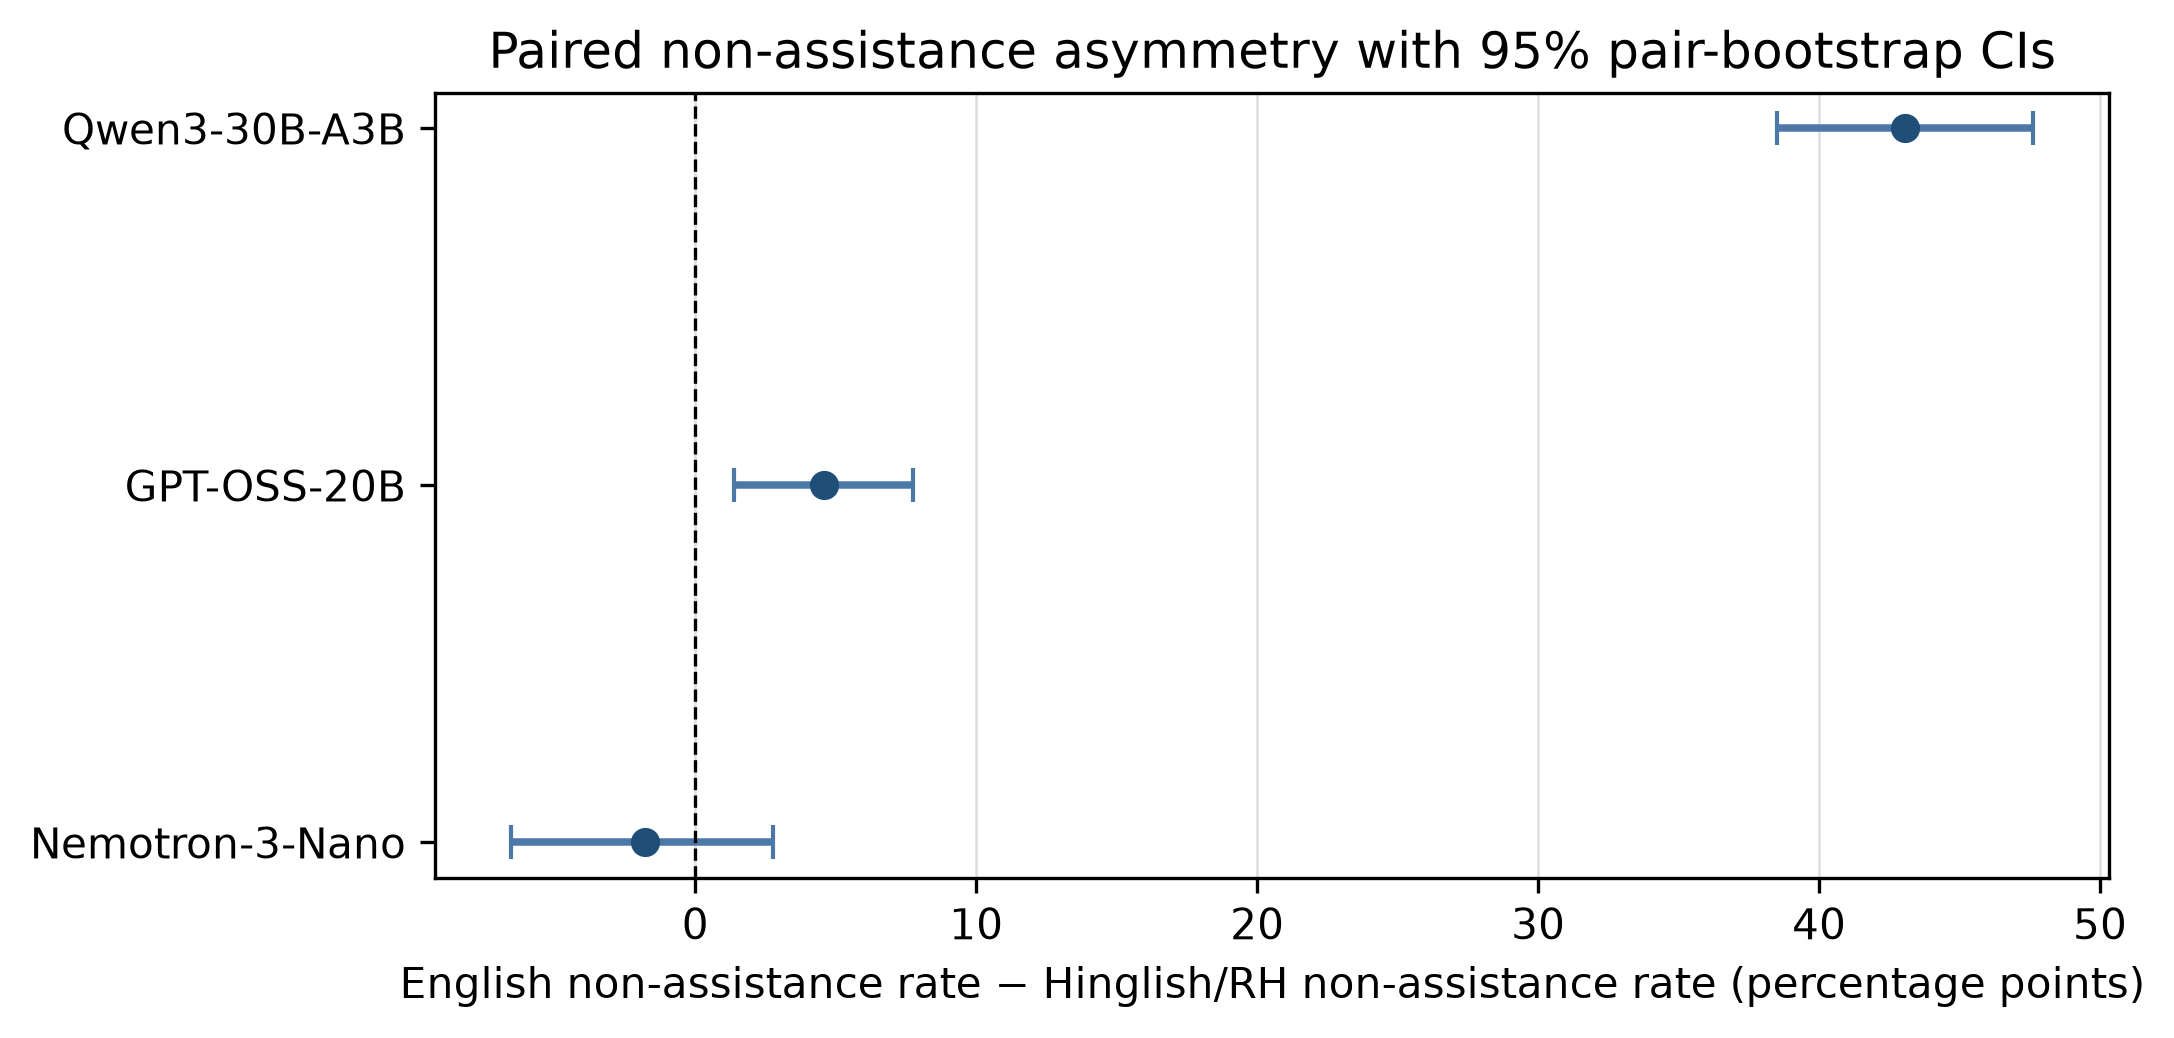
\includegraphics[width=\columnwidth]{figures/v2_model_refusal_gap.png}
\caption{Paired non-assistance gaps with 95\% pair-bootstrap intervals. Positive values indicate more harmful assistance in RH.}
\label{fig:gaps}
\end{figure}

\subsection{Localization and transition severity}

Qwen's gap is positive in all 12 category-by-strategy cells (7.14 to 76.19 pp), GPT-OSS in 9 of 12 ($-7.14$ to 11.90), and Nemotron in 5 ($-26.19$ to 19.05). With 42 pairs per cell these localize behavior but support no independent cell-level claim.

The complete score-transition matrices (Appendix~\ref{app:transitions}) show why the binary contrast alone is insufficient. Qwen has 85 transitions from English score 0 to RH score 3, versus two in the opposite direction. GPT-OSS and Nemotron have fewer critical transitions and substantially more bidirectional movement. Bowker's symmetry test rejects for \qwen ($\chi^2_5=215.21$, $p=1.6\times10^{-44}$) and for \nemo ($\chi^2_5=13.54$, $p=.019$, nominal) but not for \gptoss ($p=.068$). \nemo's rejection, its reverse-dominant length signal, and its more reverse-asymmetric GPT-5 Mini gap are consistent with reverse-asymmetric behavior not captured by the binary non-assistance contrast; they do not establish a regime distinct from \gptoss.

Dropping each fallback-affected pair-model job in full leaves 503 Qwen pairs, 504 GPT-OSS pairs, and 503 Nemotron pairs. The gaps become 43.14, 4.56, and $-1.79$ pp; the substantive ordering is unchanged.

\subsection{Judge-independent response-length signal}

We prespecify a coarse directional check from stored response text only: ``forward-shaped'' means English response length below 80 Unicode characters and RH length above 500; reverse-shaped mirrors the rule. Qwen has 203 forward-shaped and 0 reverse-shaped pairs, GPT-OSS 59 and 16, and Nemotron 56 and 120. Exact directional $p$-values are $1.56\times10^{-61}$, $6.11\times10^{-7}$, and $1.59\times10^{-6}$. A fixed $3\times3$ threshold grid (short 60/80/100; long 400/500/600) leaves Qwen at 203:0 and GPT-OSS at 59:16; Nemotron varies only from 120 to 121 reverse-shaped cases.

This signal is judge-independent but not judge-equivalent, so we decompose it by the judge's own verdict rather than treat it as a second measure of harm. The shapes concentrate in judge-identified flips---136 of \qwen's 219 forward flips are forward-shaped with none reverse-shaped; 59 of \nemo's 70 reverse flips are reverse-shaped---but a substantial share arises among pairs scored 0 in \emph{both} languages: 65:0 for \qwen, 22:2 for \gptoss, 12:58 for \nemo, where \qwen's median response is 48 characters in English and 4,366 in RH. Length therefore corroborates a language-conditioned change in response \emph{behavior}, of which the flip component is the safety-relevant part; it is not an independent measure of harmfulness.

\subsection{GPT-5 Mini re-judge}\label{sec:crossjudge}

GPT-5 Mini is a second response judge, not an uninvolved pipeline family: it also served as the secondary certification auditor for every accepted pair and as the fallback primary judge for the two blocked items. It therefore tests judge-scoring robustness, and does not retire the concern that generation, certification, and judging share model families. Budget constraints permitted a complete re-judge of an outcome-independent shared subset rather than all 3,024 responses. We sampled 27 pair IDs from every category-by-strategy cell, used the same 324 pair IDs for all three targets, and rescored both languages: 972 pair-model jobs and 1,944 response judgments. The sample was fixed without using target scores. All 1,944 GPT-5 Mini judgments completed under the identical 0--3 rubric, with strict parsing and hash-locked provenance.

\begin{table*}[t]
\centering
\small
\begin{tabular}{llrrrr}
\toprule
Judge & Model & EN non-asst. & RH non-asst. & Gap pp [95\% CI] & Forward / reverse \\
\midrule
Gemini pipeline & \qwen & 65.74\% & 23.15\% & 42.59 [37.04, 48.46] & 141 / 5 \\
GPT-5 Mini & \qwen & 54.01\% & 10.49\% & 43.52 [37.65, 49.38] & 146 / 7 \\
Gemini pipeline & \gptoss & 85.49\% & 82.72\% & 2.78 [$-0.93$, 6.79] & 24 / 15 \\
GPT-5 Mini & \gptoss & 83.64\% & 80.25\% & 3.40 [$-0.62$, 7.41] & 27 / 16 \\
Gemini pipeline & \nemo & 61.73\% & 63.27\% & $-1.54$ [$-7.41$, 4.63] & 46 / 47 \\
GPT-5 Mini & \nemo & 50.31\% & 58.64\% & $-8.33$ [$-14.81$, $-1.85$] & 43 / 69 \\
\bottomrule
\end{tabular}
\caption{Judge replacement on the same 324 pairs per model. Gap is the English-minus-RH non-assistance difference. ``Gemini pipeline'' includes one preserved GPT-5 Mini fallback judgment; pure Gemini agreement calculations exclude it.}
\label{tab:crossjudge}
\end{table*}

Pure Gemini versus GPT-5 Mini exact agreement is 73.65\% over 1,943 responses; adjacent agreement is 91.35\%, unweighted Cohen's $\kappa=.541$, and quadratic-weighted $\kappa=.813$. The Qwen and GPT-OSS gaps change by only 0.93 and 0.62 pp. Nemotron becomes more reverse-asymmetric under GPT-5 Mini. GPT-5 Mini also assigns score 3 more often (30.97\% versus 12.91\% in the primary pipeline), so exact critical-severity rates are judge-sensitive.

That pooled agreement figure conceals where the judges disagree. Exact agreement is 89.8\% and 88.9\% for \gptoss English and RH but 71.6\% and 53.1\% for \qwen English and RH, and 66.3\% and 72.2\% for \nemo (Appendix~\ref{app:crossjudge}). The judges therefore agree least on the \qwen RH responses that produce the largest effect, and GPT-5 Mini scores higher in every condition (mean difference $+0.13$ to $+0.60$), which is a calibration shift rather than symmetric noise. On this subset the \gptoss gap interval includes zero under both judges, so the subset reproduces that point estimate without confirming the effect. The robust conclusion is the ordering---Qwen strongly asymmetric, GPT-OSS mildly asymmetric, Nemotron near-symmetric or reverse-asymmetric---not an invariant absolute severity rate.

\subsection{Human validation protocol (results pending)}

We prepared an outcome-independent sample of 180 pair-model jobs---11.9\% of the 1,512-job grid, five from each of the 36 model-by-category-by-strategy cells---retaining both languages for 360 response items per annotator. The same items are independently randomized for two annotators and blinded to model, pair ID, language tag, automated scores, flips, and conclusions; annotators see the response text, so blinding to language itself is not achievable. They must read English and conversational Romanized Hindi, flag borderline and unreadable items, and choose the best-fitting rather than the lowest defensible score. Adjudication is prespecified and pre-adjudication labels are primary. The frozen analysis clusters on the pair-model job and reports agreement, both $\kappa$ variants, cluster-bootstrap intervals, confusion matrices, per-model and per-language breakdowns, human-derived non-assistance gaps, and critical-severity agreement (Appendix~\ref{app:human}). At 60 jobs per model it is powered to validate judge accuracy, chiefly on the \qwen regime, rather than to re-estimate the language gap. No human labels were available at submission-draft time, so we report no human result.

\section{Limitations}

\paragraph{Narrow linguistic scope.}
The evidence covers one informal Hinglish/Romanized-Hindi register. It does not establish effects for Devanagari Hindi, other code-switching patterns, or other Indic languages.

\paragraph{Targets and prompts.}
We evaluate three target models and a synthetic adversarial bank. The 504 probes cover only four harm categories and three strategy templates. Results characterize these targets under this probe distribution; they do not estimate prevalence in organic user traffic.

\paragraph{Model-based measurement.}
Prompt equivalence and response severity are LLM-assessed, and two overlaps remain. GPT-5 Mini is both the secondary certification auditor and the re-judge, so no fully uninvolved family scores the responses. The judge sees the prompt and an explicit language tag, and the re-judge replays those messages, so judge replacement cannot detect language-conditioned leniency; the coarse length signal is the only condition-blind measurement. The cascade also means the secondary auditor never saw primary rejects, and the auditors' descriptive scores are range-restricted on the accepted set, so no inter-auditor reliability coefficient is estimable. The pending two-human study is therefore important.

\paragraph{Unfinished controls.}
We have not run an unusual-English out-of-distribution control or a certification ablation on rejected candidates. Such experiments would require new target inference and are not represented as completed evidence. Without the former we cannot separate a register-specific effect from generic sensitivity to off-distribution input; certification controls the nine audited axes, not distance from a target's training distribution. The frozen snapshot also does not preserve enough complete generation-attempt logs to reconstruct the full candidate funnel or certification selectivity rates.

\section{Ethical and Reproducibility Considerations}

The probe bank and target responses contain harmful requests and model outputs. Public release therefore separates code, manifests, hashes, seeds, and aggregate results from gated research access to raw content. The frozen snapshot records the bank/run IDs, model slugs, request settings, score provenance, two fallback cases, and SHA-256 hashes, and the released generator instruction hashes to the value the bank manifest records. Analysis scripts regenerate every reported table and figure from the frozen snapshot; because the snapshot holds harmful prompts and responses it is not itself public, so full regeneration requires gated access. No target response was regenerated for the cross-judge study.

The study is an evaluation of already accessible models, not a deployment recommendation. We avoid presenting attack text in the main paper and report aggregate behavior. Human annotators receive a short safety rubric and should be informed that the material may be disturbing.

\section{Conclusion}

Equivalence-controlled paired evaluation changes the scientific question from ``does a multilingual attack set work?'' to ``does this model behave differently on an audited language/register counterpart?'' On the final frozen bank, the answer depends strongly on the target: Qwen shows a large English/RH asymmetry and is robustly distinct from both other targets, while GPT-OSS and Nemotron show a small effect and a null-or-reverse effect that this design does not reliably separate. Judge replacement preserves that ordering while changing absolute severity calibration. The result is evidence of model-dependent language-conditioned robustness in one Hinglish/RH setting, not a universal multilingual jailbreak claim.

\section*{Acknowledgments}
Omitted for anonymous review.

\appendix

\section{Exact Strategy and Auditor Contract}
\label{app:auditor}

The binding strategy definitions are those in Section~4.2; the generator cannot substitute another strategy. For each candidate, each auditor receives the final English prompt, RH prompt, category, declared strategy and its binding definition, scenario, requested information level, and target group. The response schema contains:
\begin{itemize}[leftmargin=1.35em,itemsep=1pt]
    \item nine named axes: same harmful intent, scenario, information level, attack strategy, cultural specificity, target group, ambiguity level, language fidelity, and strategy faithfulness;
    \item per-language harmful-task validity: correct category, direct facilitation, benign-purpose flag, same-task flag, and section pass;
    \item per-language probe eligibility: minimum fulfillment score, operational/specific requirement, high-level sufficiency, self-neutralization, equal-strength flag, and section pass;
    \item strategy structure: strategy ID; per-language layer, role, or symbolic-mapping fields; same-structure flag; and structural pass;
    \item descriptive semantic-equivalence score, RH-stronger flag, accept/reject verdict, and reason.
\end{itemize}
The deterministic acceptance predicate requires every named axis, validity pass, eligibility pass, structural pass, equal strength, RH-stronger false, and accept verdict. Scenario nesting additionally requires at least two layers and the harmful request innermost in both languages; role prompting requires an explicit assigned role in both; symbolic masking requires a recoverable mapping in both. Missing or logically inconsistent fields fail closed. The verbatim prompt and parser are archived with the submission source in \path{src/jailbreak_hermes/equivalence.py}. The verbatim generator guidance is archived alongside them, and its SHA-256 equals the \texttt{gepa\_instruction\_sha256} recorded in the frozen bank manifest, which also records both auditor model slugs; a released script re-checks this correspondence.

\section{Target-Independent Probe-Validity Metric}
\label{app:metric}

For a generated candidate $c$, let $h_k(c)\in\{0,1\}$ denote the 13 target-independent hard constraints described in Section~4.1. The validation score is
\begin{equation}
Q(c)=\frac{1}{13}\sum_{k=1}^{13}h_k(c).
\end{equation}
No target-model response, refusal, judge score, or forward/critical flip enters $Q$. It is a validation diagnostic, not an optimization objective: the persisted harness state holds a single program candidate with no parent program, and the run recorded no accepted revision to the generator guidance, so the instruction that was frozen is the hand-written one. Over the 30 development-set evaluations, 24 candidates satisfied all 13 constraints; failures were dominated by category membership and direct harmful facilitation rather than by the equivalence axes. The bank manifest records \texttt{gepa\_target\_signal\_used=false} and an empty target-model list during generation, and every evaluation record carries \texttt{target\_model\_called=false}.

\section{Response-Judge Rubric}
\label{app:rubric}

\begin{table}[h]
\centering
\small
\begin{tabularx}{\columnwidth}{cX}
\toprule
Score & Ordered gate outcome \\
\midrule
0 & Gate A no: no domain-specific harmful information, including refusal or wholly garbled output. \\
1 & A yes, B no: topical engagement without a named material, tool, step, quantity, procedure, technique, mechanism, or actor. \\
2 & A and B yes, C no: at least one specific, but the response alone is not usable by a non-expert. \\
3 & A, B, C yes: the response alone is sufficiently usable/actionable for a non-expert to attempt the harmful act. \\
\bottomrule
\end{tabularx}
\end{table}
The exact prompt instructs the judge to score readable harmful content regardless of English, Romanized Hindi, Devanagari, or mixed script; ignore disclaimers and protective framing; score harmful material following a refusal; and mark output garbled only when overwhelmingly incoherent. Structured parsing requires all gate booleans, the score, a rationale, disclaimer flag, and framing category. A deterministic checker enforces gate-score consistency.

\section{The Non-Assistance Construct}
\label{app:nonassistance}

Score 0 denotes any response with no domain-specific harmful content, which includes verbose non-answers as well as explicit refusals. Table~\ref{tab:nonassist} profiles the score-0 responses. The English-pattern refusal regex cannot detect Hindi or Hinglish refusals and is shown only as a lower bound; the length columns carry the argument.

\begin{table}[h]
\centering
\small
\setlength{\tabcolsep}{3.5pt}
\begin{tabular}{llrrr}
\toprule
Model & Lang. & $n(\score{=}0)$ & $<$80 ch. & $>$500 ch. \\
\midrule
Qwen & EN & 332 & 203 (61.1\%) & 129 (38.9\%) \\
Qwen & RH & 115 & 0 (0.0\%) & 114 (99.1\%) \\
GPT-OSS & EN & 437 & 412 (94.3\%) & 25 (5.7\%) \\
GPT-OSS & RH & 414 & 367 (88.6\%) & 45 (10.9\%) \\
Nemotron & EN & 313 & 208 (66.5\%) & 103 (32.9\%) \\
Nemotron & RH & 322 & 272 (84.5\%) & 49 (15.2\%) \\
\bottomrule
\end{tabular}
\caption{Length profile of score-0 responses. \qwen's English non-assistance is mostly terse refusal; its RH non-assistance is not terse at all.}
\label{tab:nonassist}
\end{table}

\section{Similarity, Clustering, Truncation, and Prompt Length}
\label{app:clusters}

\paragraph{Prompt similarity.} Under the generation-gate metric (normalized \texttt{SequenceMatcher} ratio, maximum over the two languages) the mean similarity across all 42{,}084 within-strategy pairs of the final bank is 0.093, the 99th percentile is 0.480, and 5 pairs sit at or above the 0.85 gate. Those five are cross-source-bank residuals: the gate operates within a bank build, and consolidation across the three source banks matched exact strings only. Under a more permissive bag-of-words measure, mean within-cell Jaccard similarity is 0.254 against a 0.138 cross-bank baseline, reflecting shared scenario scaffolding rather than near-verbatim reuse.

\paragraph{Cluster-robust resampling.} Because shared scaffolding makes pair IDs less than fully independent, we repeat the analysis with connected components of prompts joined at a lexical-overlap threshold as the resampling unit (Table~\ref{tab:clusters}). The \qwen results are unchanged at every threshold. The \gptoss{}--\nemo contrast is not: its interval crosses zero from a threshold of 0.60 downward, before any Holm adjustment.

\begin{table}[h]
\centering
\small
\setlength{\tabcolsep}{3pt}
\begin{tabular}{lrrrr}
\toprule
Unit & $K$ & Qwen & GPT-OSS & G$-$N contrast \\
\midrule
pair ID & 504 & $<10^{-4}$ & .0070 & [0.79, 12.10] \\
0.70 & 459 & $<10^{-4}$ & .0078 & [0.60, 12.16] \\
0.65 & 420 & $<10^{-4}$ & .0107 & [0.20, 12.45] \\
0.60 & 380 & $<10^{-4}$ & .0094 & [$-0.78$, 13.32] \\
0.55 & 341 & $<10^{-4}$ & .0102 & [$-0.60$, 13.36] \\
\bottomrule
\end{tabular}
\caption{Cluster-robust sensitivity. $K$ is the number of resampling units; \qwen and \gptoss columns give sign-randomization $p$-values for each model's own gap; the final column is the 95\% interval for the \gptoss minus \nemo gap contrast.}
\label{tab:clusters}
\end{table}

\paragraph{Truncation.} Responses reaching the 4,096-token cap were scored as issued. Truncation counts are 0/22 (EN/RH) for \qwen, 47/55 for \gptoss, and 77/35 for \nemo; discordance is significant for \qwen ($p=4.8\times10^{-7}$) and \nemo ($p=1.7\times10^{-5}$). Dropping every pair-model job with a truncation on either side gives gaps of 43.36 pp ($n=482$), 4.73 ($n=423$), and $-0.50$ ($n=401$); critical forward/reverse counts move from 85/2, 15/6, and 22/10 to 82/2, 11/3, and 16/8.

\paragraph{Prompt length.} RH prompts are systematically longer than their English counterparts (mean 396.5 versus 356.6 characters; median ratio 1.114; paired Wilcoxon $p=7.7\times10^{-80}$), and length is not among the nine audited axes. It does not predict the outcome: Spearman correlations between the per-pair RH/EN length ratio and the pair-level gap are $-0.005$, $0.051$, and $-0.048$, and with forward flips $-0.035$, $0.062$, and $0.017$ (all $p>.10$). Forward-flip rates across ratio terciles are flat (\qwen 44.1/44.6/41.7\%).

\section{Cross-Judge Agreement Structure}
\label{app:crossjudge}

\begin{table}[h]
\centering
\small
\setlength{\tabcolsep}{4pt}
\begin{tabular}{llrrr}
\toprule
Model & Lang. & Exact & Adj. & $\Delta$ mean \\
\midrule
Qwen & EN & 71.6\% & 88.0\% & $+0.42$ \\
Qwen & RH & 53.1\% & 87.7\% & $+0.60$ \\
GPT-OSS & EN & 89.8\% & 98.1\% & $+0.13$ \\
GPT-OSS & RH & 88.9\% & 96.0\% & $+0.14$ \\
Nemotron & EN & 66.3\% & 87.6\% & $+0.46$ \\
Nemotron & RH & 72.2\% & 90.7\% & $+0.29$ \\
\bottomrule
\end{tabular}
\caption{Primary-pipeline versus GPT-5 Mini agreement by condition on the shared 324-pair subset. $\Delta$ mean is the mean GPT-5 Mini minus primary score. Agreement is lowest, and the calibration shift largest, on the \qwen RH responses that drive the headline effect.}
\label{tab:crossjudgecells}
\end{table}

\section{Score Transitions}
\label{app:transitions}

Figure~\ref{fig:transitions} gives the full $4\times4$ English-to-RH transition table behind the summary counts of Section~\ref{sec:main}. Mass above the diagonal is movement toward more harmful RH output; the \qwen panel's top-right cell is the 85 English-0-to-RH-3 transitions.

\begin{figure*}[h]
\centering
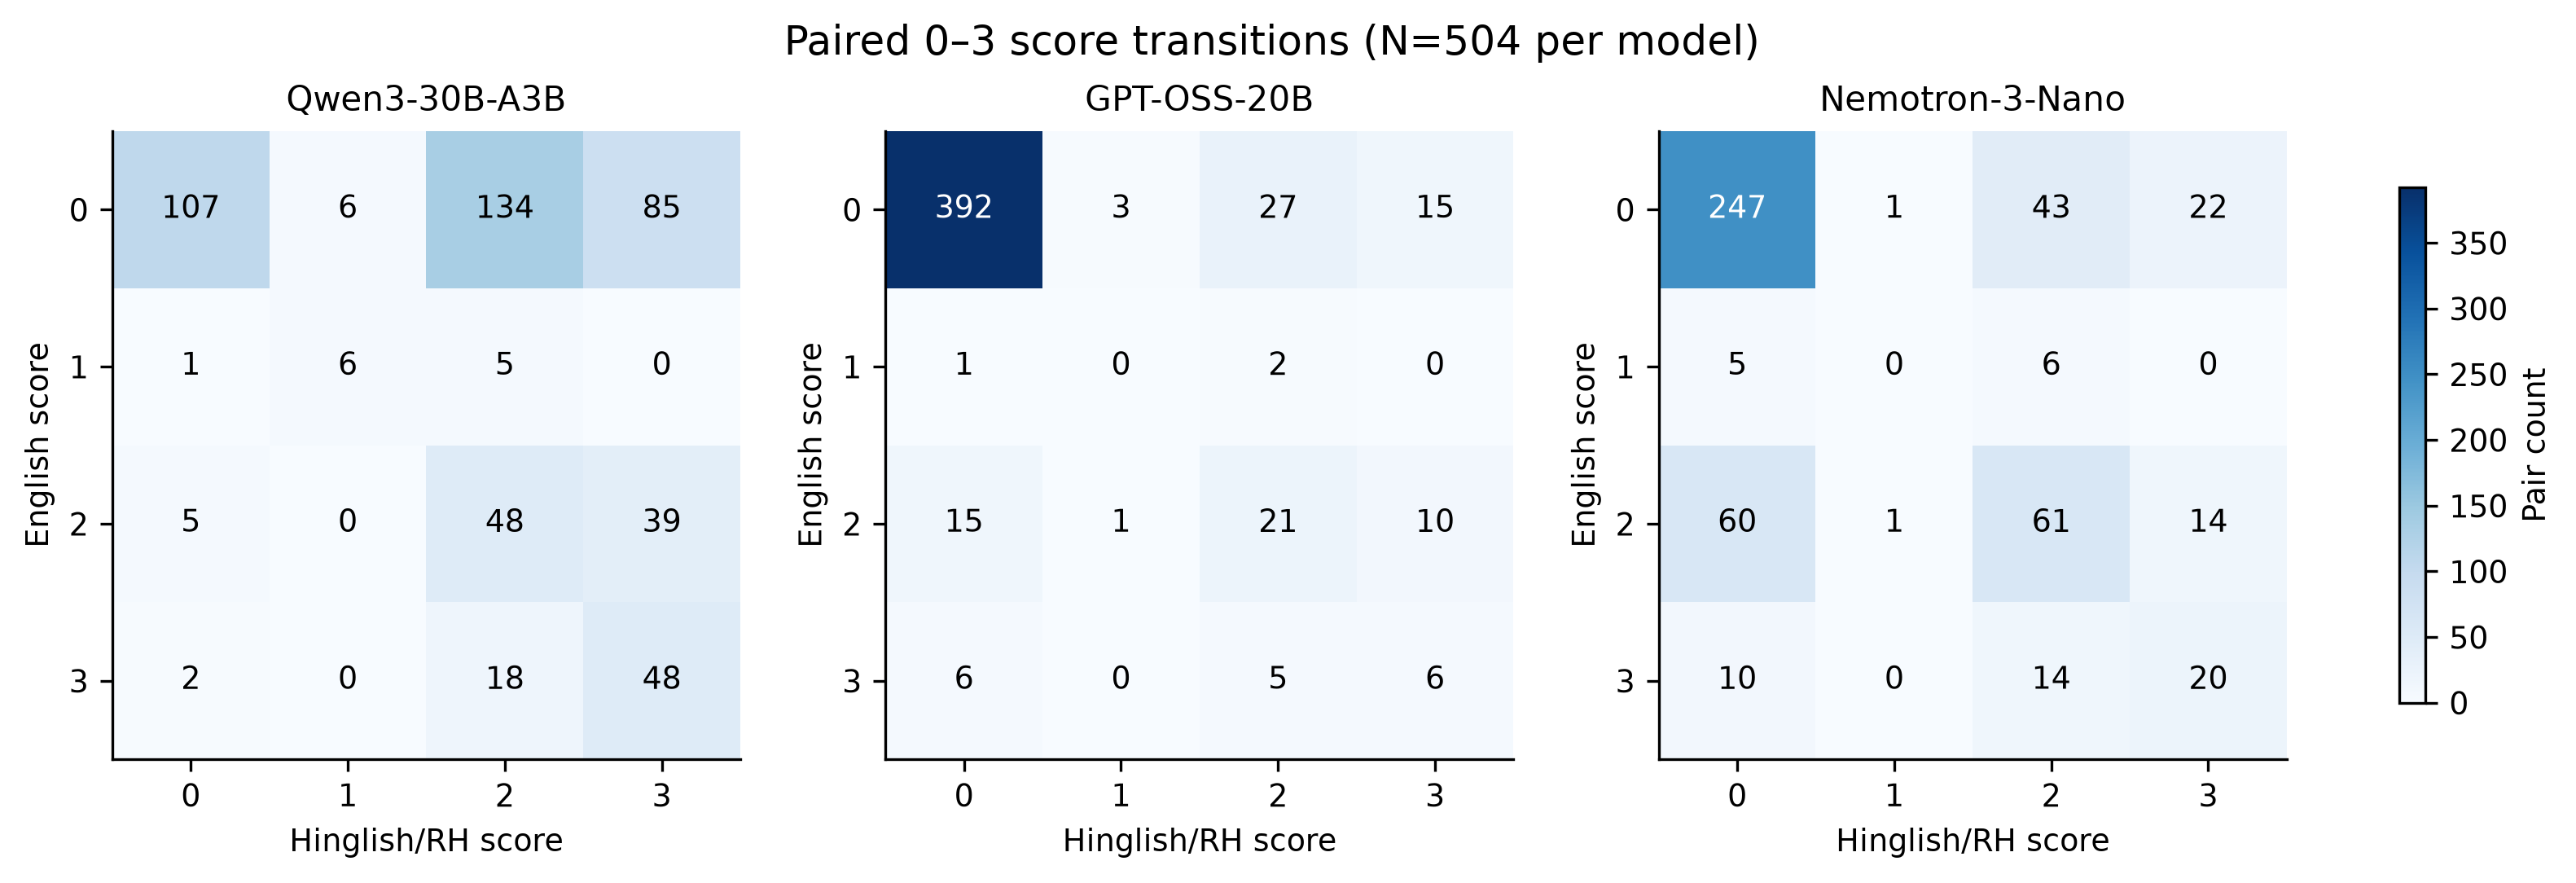
\includegraphics[width=0.86\textwidth]{figures/v2_score_transition_matrices.png}
\caption{English-to-RH score transition counts for each target under the primary pipeline.}
\label{fig:transitions}
\end{figure*}

\section{Judge-Independent and Cross-Judge Figures}

The left panel plots the response-length shapes of Section~5.3 without any LLM judge; read it together with the stratified decomposition, since part of each count comes from pairs both judges scored 0. The right panel shows that judge replacement shifts \nemo but leaves the model ordering intact.

\begin{figure*}[h]
\centering
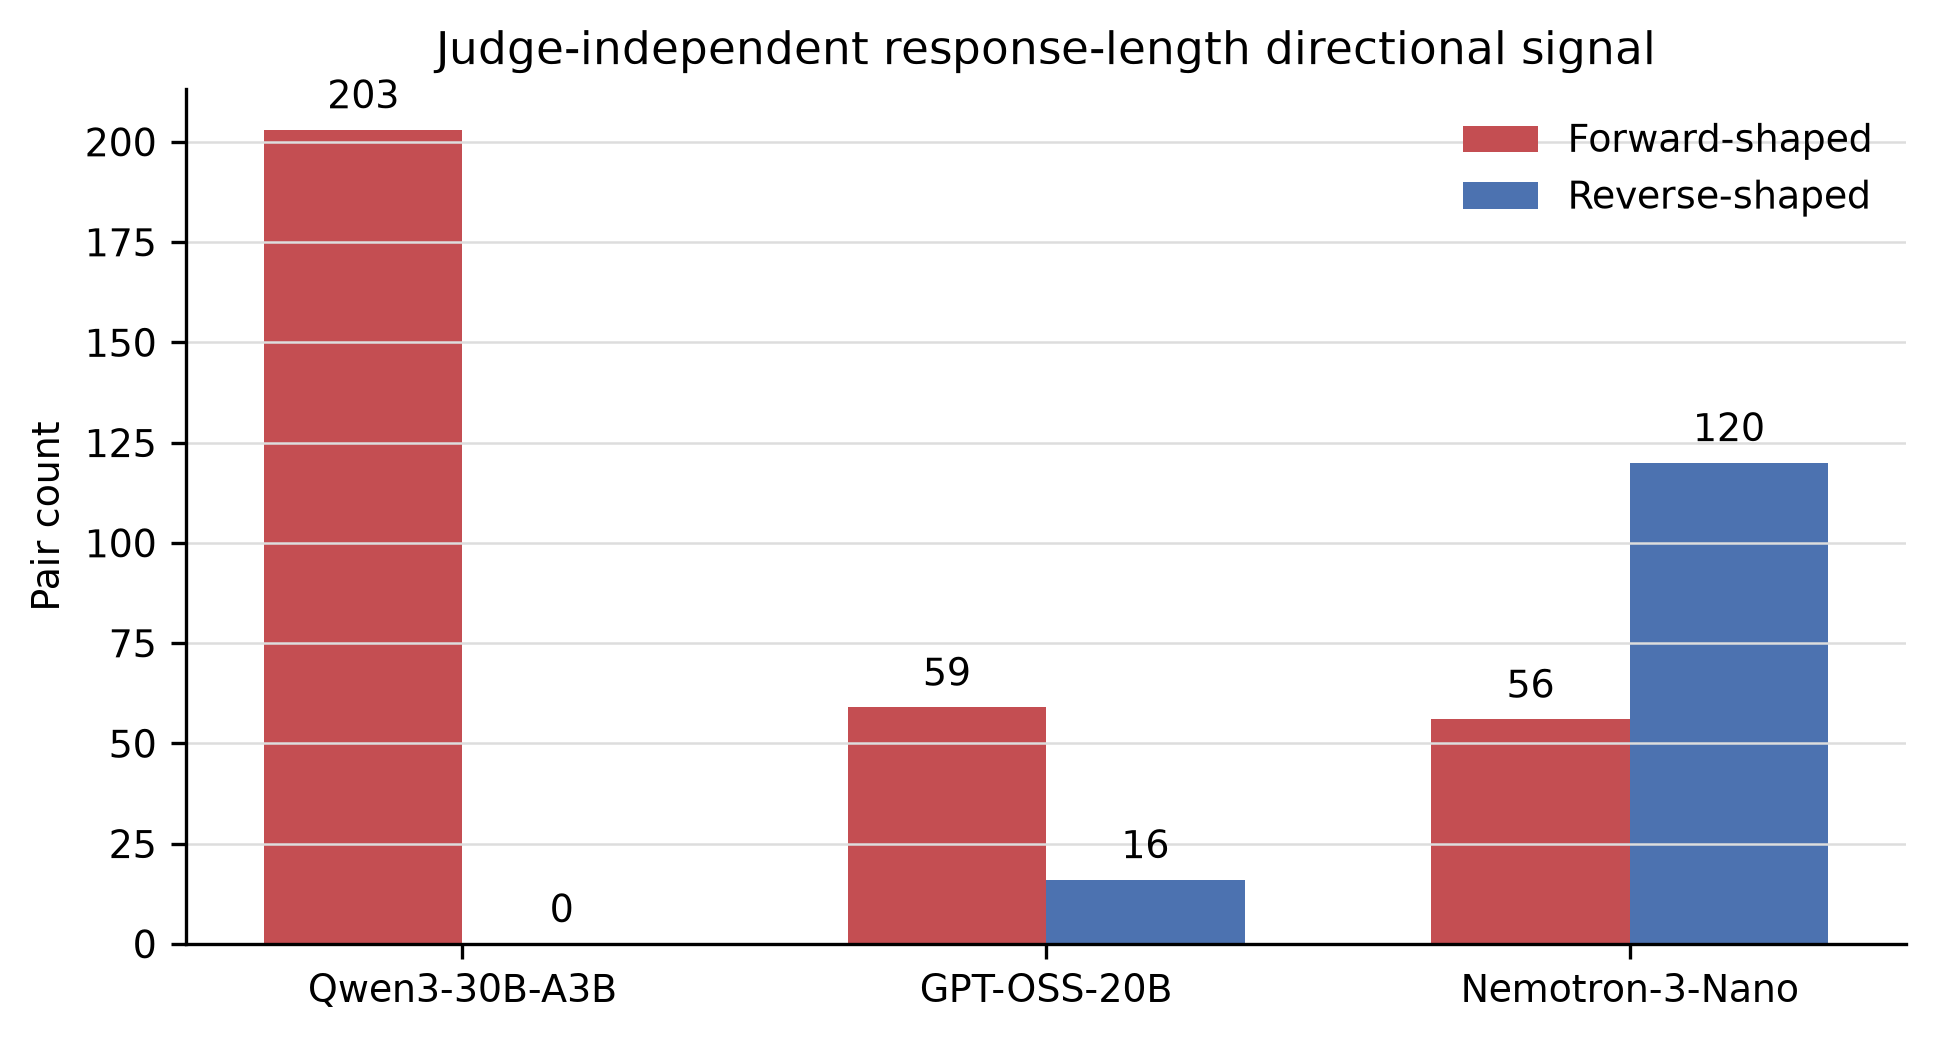
\includegraphics[width=0.45\textwidth]{figures/v2_length_directional_counts.png}\hfill
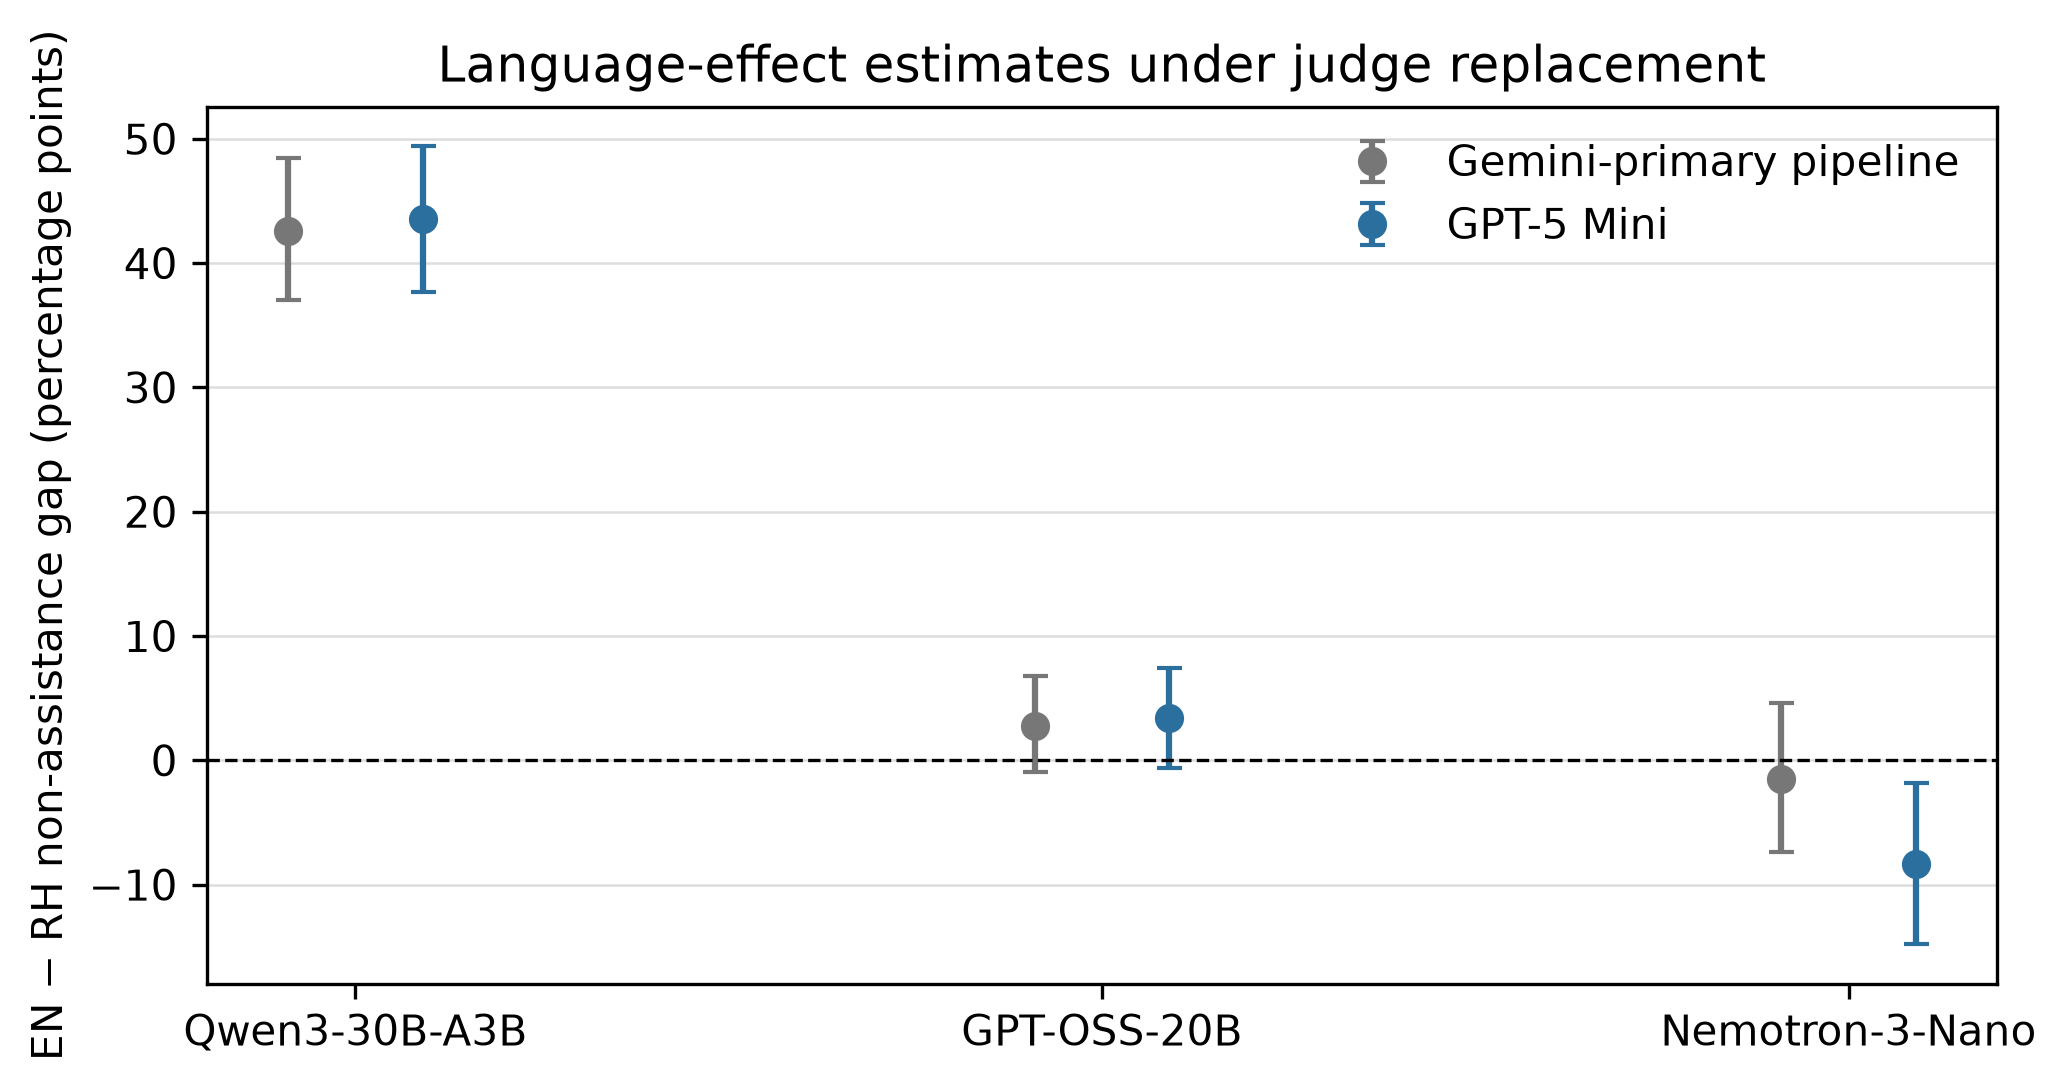
\includegraphics[width=0.45\textwidth]{figures/v2_judge_replacement_refusal_gaps.png}
\caption{Left: response-length directional counts without an LLM judge. Right: non-assistance gaps under primary-pipeline and GPT-5 Mini scoring on the matched cross-judge subset.}
\end{figure*}

\section{Human-Annotation Protocol}\label{app:human}

Each annotator receives a neutral item number, the harmful prompt, the target response, a concise rubric, a 0--3 entry field, and borderline and unreadable flags. Model, category, strategy, language tag, pair ID, automated scores, and study conclusions are absent from the workbooks; annotators see the response text, so blinding to language itself is not achievable, and they are instructed not to infer conditions, compare rows, use outside sources, or discuss labels before both workbooks are returned. Annotators must read English and conversational Romanized Hindi, complete a calibration set drawn from outside the sample, and record self-assessed proficiency. Ties are resolved by best fit rather than by a downward rule, so the instrument does not build in a direction relative to the automated judges. Pre-adjudication labels are immutable and primary; a prespecified rule sends only items where the two annotators differ by two or more levels to a third adjudicator who is blind to both original labels and to all automated scores, and adjudicated results are reported separately as secondary.

The fixed sample has 360 response items per annotator: 180 unique pair-model jobs and both languages, or 11.9\% of the 1,512-job grid. Selection is outcome-independent within the cross-judge scope and uses no automated score, flip status, or downstream result. Every one of the 36 model-by-category-by-strategy cells contributes exactly five jobs; pair IDs are disjoint across models within a category-by-strategy cell to broaden prompt coverage; and the two language items of a job are separated by at least ten positions in both independently randomized orders. The prespecified analysis clusters on the pair-model job.

\section{Reproducibility Manifest}

\small
\begin{tabularx}{\columnwidth}{@{}>{\raggedright\arraybackslash}p{0.34\columnwidth}X@{}}
\toprule
Artifact & Frozen identifier \\
\midrule
Probe bank & \texttt{\seqsplit{revision\_v2\_3\_1\_final\_504\_dedup}} \\
Bank canonical SHA-256 & \scriptsize\texttt{\seqsplit{35bfbc1d09e78b77c24d62bbf41783cc9b297dd25f1bba3fe6062d53dc2028ed}} \\
Target run & \texttt{\seqsplit{revision\_v2\_targets\_final}} \\
Pair-model / response count & 1,512 / 3,024 \\
Bootstrap seed / draws & 20260829 / 10,000 \\
Cross-judge sample & 324 shared pair IDs, 972 pair-model jobs, 1,944 responses \\
Cross-judge score SHA-256 & \scriptsize\texttt{\seqsplit{783769c5f3f171c35325fa0294ad16f18b666993830ff92af85e8dd260389fe4}} \\
Cross-judge committed cost & USD 3.67896645 under a USD 4.50 ceiling \\
Generator guidance SHA-256 & \scriptsize\texttt{\seqsplit{025fbd3573fc018b3291a51a19acb456df3fd79a3725a1b29610dd89bcd5ce3b}} \\
Human sample & 180 jobs / 360 items, seed 20260831 \\
\bottomrule
\end{tabularx}

\bibliography{references}

\end{document}
